\chapter{Introduction to Dynamic Programming}

\section{Dynamic Programming Setting}
Consider a \emph{generic} optimization problem
\[
\min_{u\in U}g(u)
\]
where $u$ is the decision variable, $g(u)$ is the cost function, and $U$ is the constraint set.
There are several categories of problems:
\begin{itemize}
\item
Discrete (i.e., $U$ is finite), or continuous
\item
Linear (i.e., $g$ is lienar and $U$ is polyhedral) or nonlinear
\item
Stochastic or deterministic: For stochastic problems, the cost involves a stochastic parameter $\omega$, which is averaged:
\[
g(u)=\mathbb{E}_{\omega}\{G(u,w)\}
\]
where $\omega$ is a random parameter.
\end{itemize}
The dynamic programming (dp) is able to deal with complex stochastic problems where $\omega$ becomes available in stages, and the decisions are also made in stages based on the information.

\subsection{Basic Structure of Stochastic DP}
The DP usually invoves the following elements:
\begin{itemize}
\item
Discrete-time system:
\[
\begin{array}{ll}
x_{k+1} = f_k(x_k,u_k,\omega_k),&k=0,1,\dots,N-1
\end{array}
\]
where
\begin{itemize}
\item
$k$ denotes the stage / discrete time
\item
$x_k$ denotes the state for stage $k$, which \emph{summarizes past information} that is relevant for future decision
\item
$u_k$ denotes the control variable, i.e., a decision to be selected at time $k$ from a given set. When making the decision, the state $x_k$ is known.
\item
$w_k$ denotes the \emph{random parameter} / \emph{disturbance} / \emph{noise} at stage $k$.
\item
$N$ is the \emph{Horizon} or the number of times that the control is applied.
\end{itemize}
\item
A cost function that is \emph{addictive} over time:
\[
\mathbb{E}\left\{
g_N(x_N)
+
\sum_{k=0}^{N-1}g_k(x_k,u_k,\omega_k)
\right\}
\]
\end{itemize}
\begin{remark}
We may use the transition matrix as the alternative \emph{discrete-system} description, i.e., suppose the transition matrix $P(x_{k+1}\mid x_k,u_k)$ is available, then
\[
x_{k+1} = \omega_k,\ \text{with }
P(\omega_k\mid x_k,u_k) = P(x_{k+1}\mid x_k,u_k)
\]
\end{remark}
Several assumptions are made for common dp problem:
\begin{itemize}
\item
The set of possible values for control $u_k$ depend at most on $x_k$ but not on \emph{prior} $x$ or $u$
\item
The probability distribution of $\omega_k$ does not depend on past values $\omega_{k-1},\dots,\omega_0$, i.e., $\omega_k\sim P(\cdot ; x_k,u_k)$, but may depend on $x_k$ and $u_k$, since otherwise past values of $\omega$ would be useful for future optimization by applying \emph{state augmentation}.
\end{itemize}

\subsection{Inventory Control Example}\label{subsec:1:1:2}
The inventory model is summarized in the figure below:
\begin{figure}
\centering
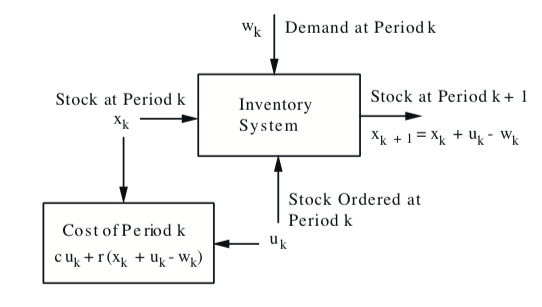
\includegraphics[width = 0.7\textwidth]{First_lecture/p_2}
\caption{Inventory Model}
\end{figure}
In this case, the discrete-time system is
\[
x_{k+1} = f_k(x_k,u_k,\omega_k) = x_k + u_k - \omega_k
\]
with the cost function that is\emph{additive} over time:
\[
\mathbb{E}\left\{
g_N(x_N)+\sum_{k=0}^{N-1}g_k(x_k,u_k,\omega_k)
\right\}
=
\mathbb{E}\left\{
\sum_{k=0}^{N-1}(c\cdot u_k + r\cdot (x_k + u_k - \omega_k))
\right\}
\]
Our goal is to optimize the cost function over \emph{policies}, and the policies $u_k = \mu_k(x_k)$ maps states into controls. The discrete-time system for this problem is deterministic, but the cost function is a expected value for a stochastic rv.


\subsection{Deterministic Finite-State Problem}\label{subsec:1:1:3}
Consider a deterministic dp problem. We aim to find the optimal sequence of four operations $A,B,C,D$, where $A$ must \emph{precede} $B$ and $C$ must \emph{precede} $D$. Assume the startup cost to be $S_A,S_C$, and the setup transition cost from operation $m$ to operation $n$ is $C_{mn}$.

We may list all possible scheduling in the figure below:
\begin{figure}
\centering
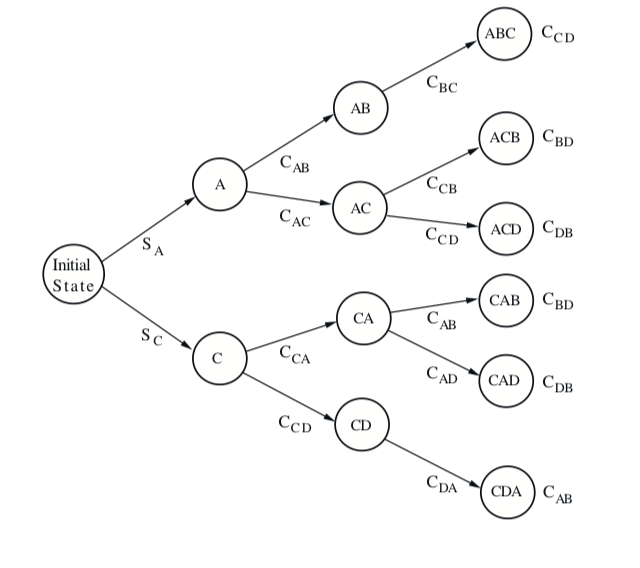
\includegraphics[width = 0.7\textwidth]{First_lecture/p_3}
\caption{Scheduling Problem}
\end{figure}

The discrete-time system for this problem is deterministic, and the cost function is deterministic as well.

\subsection{Stochastic Finite-State Problem}
The goal is to find the two-game chess match strategy. 
\begin{itemize}
\item
The \emph{timid} play draws with probability $p_d>0$ and loses with probability $1-p_d$
\item
The \emph{bold} play wins with probability $p_w<\frac{1}{2}$ and loses with probability $1-p_w$.
\end{itemize}
We may list all possible strategies result in the figure~(\ref{fig:1:3}).
\begin{figure}
\centering
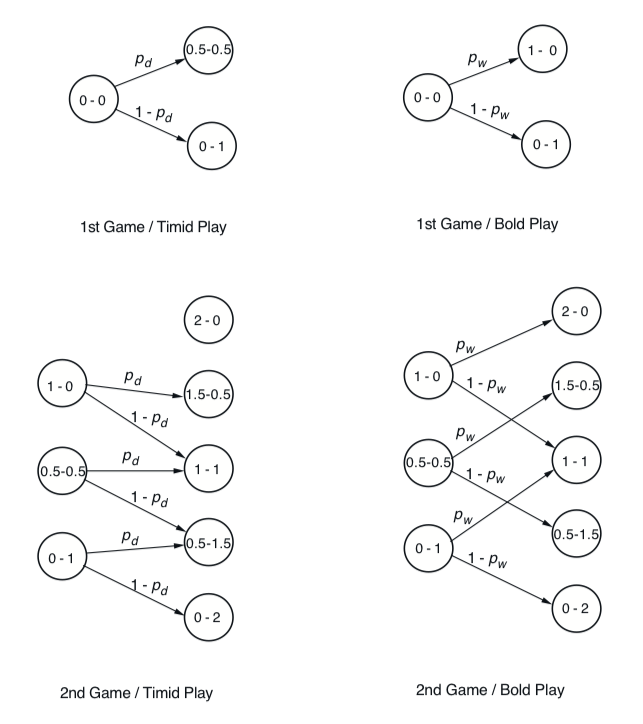
\includegraphics[width = 0.9\textwidth]{First_lecture/p_4}
\caption{Two-Game Chess Match Strategies}
\label{fig:1:3}
\end{figure}
The discrete-time system for this problem is stochastic, and the cost function is stochastic as well.

\subsection{Formal Setting of DP}
The formal setting of DP is as follows:
\begin{itemize}
\item
The system transition satisfies
\[
\begin{array}{ll}
x_{k+1} = f(x_k,u_k,\omega_k),&k=0,1,\dots,N-1
\end{array}
\]
\item
The control constraints only depends on $x_k$, i.e., $u_k\in U_k(x_k)$
\item
The probability distribution of $\omega_k$ is $P_k(\cdot\mid x_k,u_k)$
\item
The policy is a collection of functions $\pi = \{\mu_0,\dots,\mu_{N-1}\}$, where $\mu_k$ maps states $x_k$ into controls $u_k = \mu_k(x_k) \in U_k(x_k)$ for all $x_k$
\item
The expected cost of $\pi$ starting at $x_0$ is given by
\[
J_{\pi}(x_0)
=
\mathbb{E}
\left\{
g_N(x_N)+\sum_{k=0}^{N-1}g_k(x_k,\mu_k(x_k),\omega_k)
\right\}
\]
The goal is to minimize the cost function:
\[
J^*(x_0) = \min_{\pi}J_{\pi}(x_0),
\]
where the optimal policy $\pi^*$ satisfies
\[
J_{\pi^*}(x_0) = J^*(x_0).
\]
Note that $\pi^*$ is independent of $x_0$.
\end{itemize}

\subsection{Significance of Feedback}
The closed-loop policies refer to that the controller can adapt to the unexpected values of the state, while the open-loop policies cannot get access to this information.
\begin{itemize}
\item
For deterministic problems, the \emph{open-loop policies} is as good as the \emph{closed-loop policies}
\item
For stochastic problems, the reduction in the cost gained by closed-loop is called the \emph{value of information}.
\end{itemize}

For example. consider the chess match problem,
\begin{enumerate}
\item
The probability of win using optimal open-loop policy is
\[
p_w^2 + p_w(1-p_w)\cdot \max(2p_w,p_d)
\]
\item
The probability of win using optimal closed-loop policy is
\[
p_w^2(2-p_2) + p_w(1-p_w)\cdot p_d
\]
\item
Therefore, we see that the value of information is sometimes positive:
\[
\text{Value of Information }= p_w(1-p_w)\min(p_w,p_d-p_w)
\]
\end{enumerate}
\paragraph{Variants of DP}
In the second-half of this couse, we may consider several variants of DP problems:
\begin{itemize}
\item
Continuous-time problems
\item
Imperfect state information problems
\item
Infinite horizon problems
\item
Suboptimal Control
\end{itemize}


\section{Dynamic Programming Solving}
\subsection{Principle of Optimality}
Suppose $\pi^*=\{\mu_0^*,\dots,\mu_{N-1}^*\}$ be optimal policy. Consider the \emph{tail subproblem}, i.e., we are at $x_i$ at time $i$ and wish to minimize the \emph{cost-to-go} from time $i$ to time $N$:
\[
\mathbb{E}\left\{
g_N(x_N)
+
\sum_{k=i}^{N-1}g_k(x_k,\mu_k(x_k),\omega_k)
\right\}
\]
Consider the \emph{tail policy} $\{\mu^*_i,\mu_{i+1}^*,\dots,\mu_{N-1}^*\}$.
\begin{theorem}[Principle of Optimality]
The tail policy is optimal for the tail subproblem, i.e., the optimization of the future does not depend on what we did in the past.
\end{theorem}
\begin{remark}
Consider an auto travel analogy. Suppose that the fastest route from A to C passes the place B. The principle of optimality highlights that \emph{the B to C portion of the route is also the fastest route of the trip that starts from B and ends at $C$}.
\end{remark}

The DP aims to solve all tail subproblems of $N$ horizons. The DP algorithm is based on the idea as follows:
It proceeds sequentially, by solving all the tail subproblems of a given time length, based on the solution of the tail subproblems of shorter time length.


\subsection{DP algorithm for scheduling problem}
Consider the scheduling problem discussed in subsection~(\ref{subsec:1:1:3}). The startup cost and transition cost is summarized in the figure~(\ref{fig:1:1:4}).
\begin{figure}
\centering
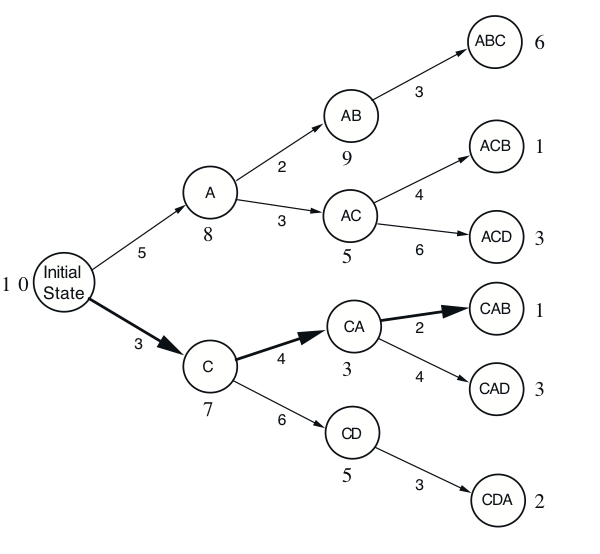
\includegraphics[width = 0.7\textwidth]{First_lecture/p_5}
\caption{Scheduling Problem Cost Description}
\label{fig:1:1:4}
\end{figure}

\paragraph{Tail Problem of Length 1: }
The subproblems involving one operations are trival to solve. State ABC,ACB,ACD,CAB,CAD,CDA correspond to the tail cost $6,1,3,1,3,2$.
\paragraph{Tail Problem of Length 2: }
Solving the subproblems involving two operations is based on the tail problem of length $1$. State $AB,AC,CA,CD$ corresponds to the tail cost $9,\min(4+1,6+3)=5,\min(2+1,4+3)=3,5$.
\paragraph{Tail Problem of Length 3: }
Solving the subproblems involving three operations is based on the tail problem of length $2$. State $A,C$ corresponds to the tail cost $\min(2+9,3+5)=8,\min(4+3,6+5)=7$.
\paragraph{Tail Problem of Length 4: }
Solving the subproblems involving four operations is based on the tail problem of length $3$. The initial state corresponds to the tail cost $\min(5+8,3+7)=10$.

After computing the optimal cost, we construct the optimal solution by starting at the initial node and proceeding forward, where each time we choose the operation that starts the \emph{optimal} schedual for the corresponding \emph{tail subproblem}. Therefore, at each state-time pair, we need to record both the optimal cost-to-go and the optimal decision.

\subsection{Stochastic Inventory Example}
Consider the inventory problem in subsection~(\ref{subsec:1:1:2}). The tail subproblems of length 1 aims to solve
\[
J_{N-1}(x_{N-1}) = \min_{u_{N-1}\ge0}\mathbb{E}_{\omega_{N-1}}
\{
c\cdot u_{N-1} + r\cdot(x_{N-1} + u_{N-1} - \omega_{N-1})
\},\ \forall x_{N-1}
\]
The tail subproblems of length $N-k$ aims to solve
\[
J_{k}(x_{k}) = \min_{u_{k}\ge0}\mathbb{E}_{\omega_{k}}
\{
c\cdot u_{k} + r\cdot(x_{k} + u_{k} - \omega_{k}) + J_{k+1}(x_k+u_k-\omega_k)
\},\ \forall x_{k}
\]
Here $J_0(x_0)$ is the optimal cost with initial state $x_0$.

\subsection{Formal Dynamic Programming Algorithm}
The dynamic programming aims to find the policy by starting with
\[
J_N(x_N) = g_N(x_N),
\]
and go backwards in time from period $N-1$ to period $0$:
\begin{equation}\label{Eq:1:1}
J_k(x_k) = \min_{u_k\in U_k(x_k)}\mathbb{E}_{\omega_k}
\left\{
g_k(x_k,u_k,\omega_k)
+
J_{k+1}(f_k(x_k,u_k,\omega_k))
\right\},\ k=0,\dots,N-1.
\end{equation}

In such case, $J_0(x_0)$ is generated at the last step, and is equal to the optimal cost $J^*(x_0)$. 
Furthermore, if $u_k^* = \mu_k^*(x_k)$ minimizes the RHS of (\ref{Eq:1:1}) for each $x_k$ and $k$, then $\pi^*=\{\mu_0^*,\dots,\mu_{N-1}^*\}$ is optimal.
\begin{proof}
Proof by induction that $J_k(x_k)$ is equal to $J_k^*(x_k)$, which is defined as the optimal cost of the tail subproblem that starts tat time $k$ at state $x_k$.
\end{proof}

\subsection{Linear-Quadratic Analytic Example}
Consider a certain material is passed through a sequence of two ovens shown in Figure~(\ref{fig:1:1:6}).
\begin{figure}
\centering
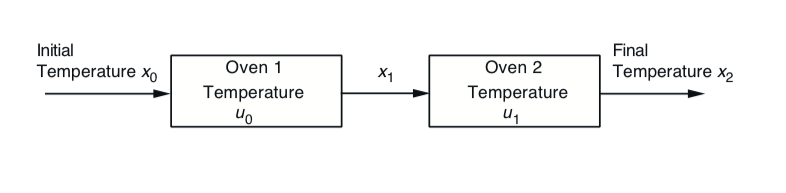
\includegraphics[width = 0.9\textwidth]{First_lecture/p_6}
\caption{Linear-Quadratic Example}
\label{fig:1:1:6}
\end{figure}
\begin{itemize}
\item
The system is given by
\[
x_{k+1} = (1-a)x_k + au_k,\quad k=0,1,
\]
where $a$ is a given scalar from the interval $(0,1)$.
\item
Define the cost function
\[
r(x_2-T)^2+u_0^2+u_1^2
\]
where $r$ is a given positive scalar.
\item
We may apply the dp algorithm as follows:
\begin{align*}
J_2(x_2)&=r(x_2-T)^2\\
J_1(x_1)&=\min_{u_1}\left[u_1^2+r((1-a)x_1 + au_1 - T)^2\right]\\
J_0(x_0)&=\min_{u_0}\left[u_0^2+J_1((1-a)x_0+au_0)\right]
\end{align*}
\end{itemize}


\subsection{State Augmentation}
When the assumptions of the basic problem are violated, then we need to consider reformulating the state. The DP algorithm still applies, but the problem gets bigger.
\paragraph{Example}
Consider the system becomes
\[
x_{k+1} = f_k(x_k,x_{k-1},u_k,\omega_k)
\]
Introducing the additional state variable $y_k = x_{k-1}$ and view $\tilde{x_k} = (x_k,y_k)$. Therefore, the new system takes the form
\[
\begin{pmatrix}
x_{k+1}\\y_{k+1}
\end{pmatrix}=\begin{pmatrix}
f_k(x_k,y_k,u_k,\omega_k)\\x_k
\end{pmatrix}
\]
The DP algorithm applies to the reformulated problem:
\[
J_k(x_k,x_{k-1})=\min_{u_k\in U_k(x_k)}\mathbb{E}_{\omega_k}
\left\{
g_k(x_k,u_k,\omega_k)
+
J_{k+1}(f_k(x_k,x_{k-1},u_k,\omega_k),x_k)
\right\}
\]
















